\documentclass{article}
% using timesnew roman
\usepackage{mathptmx}

\usepackage{geometry}
 \geometry{
 a4paper,
 left=40mm,
 right=30mm,
 top=30mm,
 bottom=30mm,
 }

\usepackage{float}
\usepackage{graphicx}
\usepackage{indentfirst}
\usepackage{hyperref}

\usepackage{tikz}
\usetikzlibrary{shapes.geometric, arrows}

\tikzstyle{startstop} = [rectangle, rounded corners, minimum width=3cm, minimum height=1cm,text centered, draw=black, fill=red!30]
\tikzstyle{io} = [trapezium, trapezium left angle=70, trapezium right angle=110, minimum width=2.5cm, minimum height=1cm, text centered, draw=black, fill=blue!30, text width=2cm]
\tikzstyle{process} = [rectangle, minimum width=3cm, minimum height=1cm, text centered, draw=black, fill=orange!30]
\tikzstyle{decision} = [diamond, minimum width=3cm, minimum height=1cm, text centered, draw=black, fill=green!30]
\tikzstyle{arrow} = [thick,->,>=stealth]
\tikzstyle{double-arrow} = [thick,<->,>=stealth]


%citation
\usepackage[backend=biber, sorting=none]{biblatex}
\addbibresource{daftar_pustaka.bib}
\graphicspath{ {./images/} }
\renewcommand*\contentsname{Daftar Isi}
\renewcommand{\figurename}{Figur}



\begin{document}
  \begin{titlepage}
    \begin{center}
      
      \null
      {
      	\LARGE \bfseries MAKALAH}\\
      [0.5cm]
      {\Large Sistem Pembantu Deteksi Penggunaan Masker yang Baik dan Benar Menggunakan Object Detection Faster R-CNN}\\
          
      \vspace{2cm}

      \begin{figure}[H]
        \centering
        
\includegraphics[width=200px]{/logo/Lambang UGM.jpg}
      \end{figure}
          
      \vspace{3cm}
    
      {\Large 
      Disusun oleh Tim \bfseries Yakuy 2} {\Large :\\
      \vspace{0.5cm}
      Ardacandra Subiantoro (18/427572/PA/18532)\\
      Arief Pujo Arianto (18/430253/PA/18766)\\
      Chrystian (18/430257/PA/18770)\\
      }


      \vspace{2cm}

      {\normalsize \bfseries
      PROGRAM STUDI S1 ILMU KOMPUTER\\
      DEPARTEMEN ILMU KOMPUTER DAN ELEKTRONIKA\\
      FAKULTAS MATEMATIKA DAN ILMU PENGETAHUAN ALAM\\
      UNIVERSITAS GADJAH MADA\\
      YOGYAKARTA\\
      \vspace{0.2cm}
      2020
      }
            
    \end{center}
  \end{titlepage}

  \pagenumbering{gobble}

  \newpage
  \pagenumbering{arabic}
  \textbf{Abstrak.} 
  \newpage
  \tableofcontents
  \newpage
  \section{Pendahuluan}
  	\subsection{Latar Belakang}
	  	Meskipun berbagai penanganan sudah dilakukan tetapi hingga hari ini jumlah kasus COVID-19 terus meningkat. Jumlah kasus total COVID-19 di seluruh dunia sudah mencapai lebih dari 48 juta kasus, dengan lebih dari 1,2 juta kematian akibat COVID-19. Kasus COVID-19 di Indonesia sudah mencapai lebih dari 400 ribu dengan lebih dari 14 ribu kematian. Dampak negatif dari pandemi COVID-19 ini sangat terasa di Indonesia. Direktur Jenderal Pajak Kementerian Keuangan (Kemenkeu) Suryo Utomo membagi dampak pandemi COVID-19 menjadi tiga garis besar \cite{zuraya}. Dampak pertama adalah membuat konsumsi rumah tangga atau daya beli yang merupakan penopang 60 persen terhadap ekonomi jatuh cukup dalam. Hal ini dibuktikan dengan data dari BPS yang mencatatkan bahwa konsumsi rumah tangga turun dari 5,02 persen pada kuartal I 2019 ke 2,84 persen pada kuartal I tahun ini. Dampak kedua yaitu pandemi menimbulkan adanya ketidakpastian yang berkepanjangan sehingga investasi ikut melemah dan berimplikasi pada terhentinya usaha. Dampak ketiga adalah seluruh dunia mengalami pelemahan ekonomi sehingga menyebabkan harga komoditas turun dan ekspor Indonesia ke beberapa negara juga terhenti.
	  	
	  	\par Dengan melemahnya ekonomi di Indonesia ini, banyak perusahaan juga sudah mulai untuk membuka kembali bisnis mereka seperti semula. Berbagai upaya pengawasan pun dilakukan agar setiap orang dapat beraktivitas seperti semula dengan aman tanpa adanya ketakutan tertular COVID-19. Tetapi meskipun berbagai cara pengawasan sudah dilakukan, masih banyak orang yang tidak mematuhi aturan dan tetap beraktivitas seperti biasa. Perlunya banyak pengawasan untuk memperingatkan kembali aturan yang ada di era \textit{new normal} ini adalah salah satu cara agar semua dapat beraktivitas kembali seperti semula serta mengurangi resiko tertular COVID-19.
	  	
	  	\par Tetapi untuk mewujudkan era \textit{new normal} ini dengan baik dan efektif, dibutuhkan pengawasan serta himbauan peraturan era \textit{new normal} ini secara skala besar dan umum sehingga dibutuhkannya banyak sekali tenaga kerja. Namun menggunakan tenaga manusia bukanlah jawaban yang tepat karena tidak efesien serta sangat sulit dan juga menyita banyak waktu apabila tenaga manusia ini mengawasi serta menghimbau setiap orang yang ada.
  	\subsection{Rumusan Masalah}
  		Berdasarkan latar belakang tersebut permasalahan utama yang akan ditelusuri ialah :
  		\begin{enumerate}
  			\item Bagaimana penambangan data dapat membantu mewujudkan dan menegakkan aturan pada era \textit{new normal} untuk dapat mengurangi penyebaran COVID-19 yang ada ?
  			\item Bagaimana cara model dapat mendeteksi serta membedakan pemakaian masker yang baik dan benar ?

  		\end{enumerate}
  	\subsection{Batasan Masalah}
  		Batasan masalah yang akan kami gunakan adalah sebagai berikut :
  		\begin{itemize}
  			\item Dataset yang akan digunakan dibatasi pada Kaggle Face Mask Detection milik Larxel\cite{larxel_2020}.
  			\item Jenis gambar yang akan diklasifikasi dibatasi pada memakai masker, tidak memakai masker, dan memakai masker yang tidak benar.
  			\item Metode penambangan data yang akan kami gunakan adalah Real-time Object Detection dengan Arsitektur Faster R-CNN\cite{NIPS2015_14bfa6bb}.
  		\end{itemize}
  \section{Tujuan dan Manfaat}
  		\par Tujuan utama, kami mengusulkan menggunakan model Object Detection dengan arsitektur Faster R-CNN untuk membantu mengawasi dan menghimbau penggunaan masker yang benar di tempat umum. Object Detection dengan menggunakan Faster R-CNN ini diharapkan dapat dengan baik membedakan dan mengklasifikasi penggunaan masker dengan baik dan juga dapat secara cepat melakukan klasifikasi tersebut.
  		
  		\par Tujuan kedua, dari hasil penambangan data kami bertujuan untuk langsung memakai model tersebut diimplementasikan langsung dengan teknologi serta kesiapa infrastruktur yang ada. Implementasi ini diharapkan dapat membantu tenaga manusia untuk dapat secara otomatis memperingatkan selalu penggunaan masker di tempat umum supaya era \textit{new normal} dapat terwujudkan. Manfaat yang kami harapkan adalah peningkatan kesadaran penggunaan masker dan kemudahan bagi tenaga manusia untuk mengawasi penggunaan masker.
  \section{Metode}
  	\subsection{Pembelajaran Model}
  	 \subsubsection{Faster R-CNN}
  	 \par Faster R-CNN pertama kali dipublikasikan pada tahun 2015. Jaringan pendeteksi objek sebelum Faster R-CNN menggunakan algoritma proposal wilayah untuk membuat hipotesis lokasi objek. Jaringan seperti R-CNN dan Fast R-CNN menggunakan algoritma berbasis CPU seperti Algoritma Selective Search yang membutuhkan waktu sekitar 2 detik untuk setiap gambar. Jaringan Faster R-CNN memperbaiki masalah ini dengan menggunakan convolutional network untuk menghasilkan proposal wilayah. Perubahan ini mengurangi waktu penghitungan proposal wilayah dari 2 detik menjadi 10 militdetik dan meningkatkan representasi fitur. Faster R-CNN terdiri dari detection pipeline yang menggunakan RPN sebagai algoritma proposal wilayah dan Fast R-CNN sebagai jaringan detektor.\cite{shilpa_2020}
  	 
  	 \begin{figure}[H]
  	 	\centering
  	 	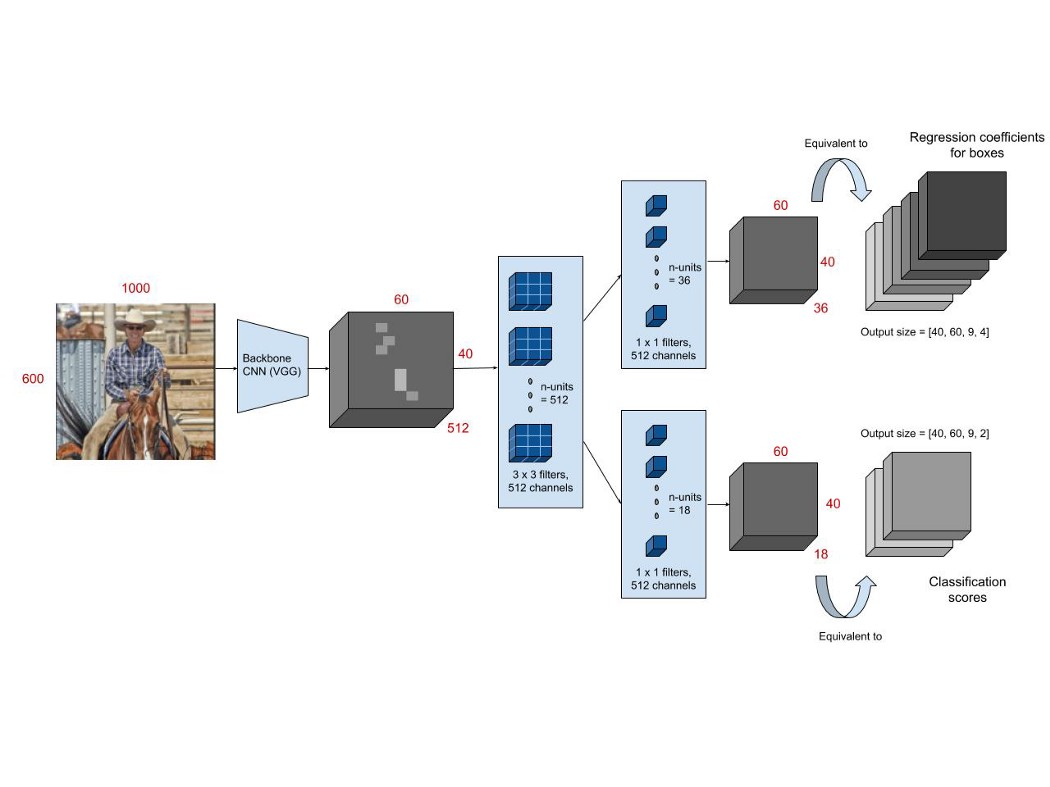
\includegraphics[width=300px]{arsitektur/RPN.jpeg}
  	 	\caption{Arsitektur RPN}
  	 \end{figure}
   
  	 \par RPN (Region Proposal Network) dimulai dengan memasukkan gambar input ke dalam Backbone CNN. Gambar input diubah ukurannya sehingga sisi yang pendek 600px dan sisi yang panjang tidak lebih dari 1000px. Output dari Backbone CNN biasanya jauh lebih kecil dari ukuran gambar input, tergantung parameter stride dari Backbone CNN. Contoh Backbone CNN yang dapat digunakan adalah jaringan VGG atau ZF-Net dengan stride 16. Hal ini berarti pixel-pixel yang bersebelahan pada output jaringan sama dengan dua pixel yang terpisah sejauh 16 pixel pada gambar input. 
  	 
  	 \par Untuk setiap titik pada output feature map, jaringan harus belajar apakah objek terdeteksi pada gambar input pada lokasi tersebut dan mengestimasi ukurannya. Hal ini dilakukan dengan meletakkan "Anchors" pada gambar input untuk setiap lokasi pada output feature map. "Anchors" mengindikasikan objek-objek yang mungkin terdapat pada lokasi tersebut dengan beragam ukuran dan aspect ratio. 
  	 
  	 \begin{figure}[H]
  	 	\centering
  	 	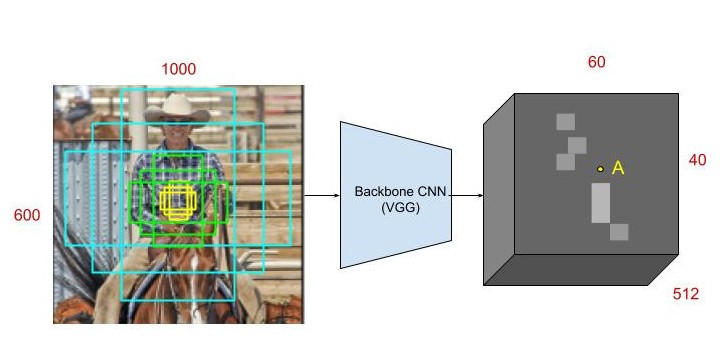
\includegraphics[width=300px]{arsitektur/contoh_anchor.jpeg}
  	 	\caption{Contoh "Anchors" pada Gambar Input dari Lokasi Titik A pada Feature Map}
  	 \end{figure}
   
   	\par Jaringan bergerak melewati setiap pixel pada output feature map dan memeriksa apakah "anchors" yang mencakupi sebuah area pada gambar input mengandung objek atau tidak, lalu mengoptimalkan koordinat-koordinat "anchors" untuk menghasilkan kotak-kotak pembatas yang disebut proposal wilayah.
   	
   	\par Konvolusi 3x3 dengan 512 unit diaplikasikan ke feature map untuk menghasilkan 512-d feature map untuk setiap lokasi. Lalu diikuti oleh 1x1 convolution layer dengan 18 unit untuk klasifikasi objek, dan 1x1 convolution dengan 36 unit untuk regresi kotak pembatas. 18 unit dari cabang klasifikasi akan mengeluarkan output dengan ukuran (H, W, 18) yang memberikan probabilitas apakah setiap titik dalam backbone feature map mengandung objek atau tidak di dalam semua 9 "anchors" pada titik. 36 unit dari cabang regresi akan mengeluarkan output dengan ukuran (H, W, 36) yang memberikan 4 koefisien regresi  untuk setiap 9 "anchors" untuk setiap titik dalam backbone feature map. Koefisien regresi meningkatkan akurasi koordinat "anchors" yang mengandung objek.
   	
   	\par Output feature map terdiri dari 40x60 lokasi, dengan total "anchors" sekitar 20 ribu. Ketika melatih model, semua "anchors" yang melewati batas gambar dihiraukan supaya tidak berkontribusi dalam penghitungan loss. Sebuah "anchor" dianggap sampel positif bila memenuhi salah satu kondisi :
   	\begin{enumerate}
   		\item "Anchor" memiliki IoU (Intersection over Union) tertinggi dengan kotak groundtruth.
   		\item "Anchor" memiliki IoU lebih besar dari 0.7 untuk setiap kotak groundtruth.
   	\end{enumerate}
   	Sebuah "anchor" dianggap sampel negatif bila IoU dengan semua kotak groundtruth kurang dari 0.3. "Anchor" yang tidak termasuk positif dan negatif akan dihiraukan saja.
   	
   	\par Setiap mini-batch untuk melatih RPN berasal dari sebuah gambar. 128 sampel positif dan 128 sampel negatif dipilih secara acak untuk menghasilkan batch. Training loss dari RPN adalah multi-task loss yang dihitung sebagai berikut : 
   
   	\begin{figure}[H]
   		\centering
   		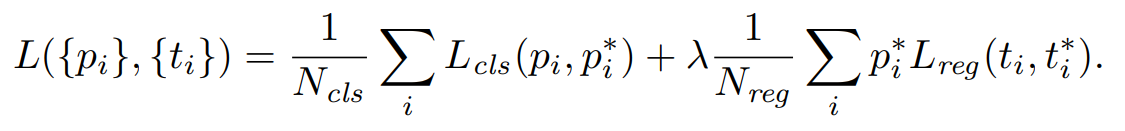
\includegraphics[width=400px]{rumus/training_loss.png}
   	\end{figure}
   
   	$i$ adalah index dari "anchor" dalam mini-batch. Classification loss adalah log loss dari dua kelas (objek vs bukan objek). $p_{i}$ adalah nilai output dari cabang klasikasi untuk "anchor" $i$, dan $p_{i}^{*}$ adalah label groundtruth.
   	
   	\par Regression loss diaktivasi hanya jika "anchor" mengandung objek. $t_{i}$ adalah output prediksi dari cabang regresi dan terdiri dari 4 variabel [$t_{x}, t_{y}, t_{w}, t_{h}$]. Regression target dihitung dengan rumus berikut :
   	
   	\begin{figure}[H]
   		\centering
   		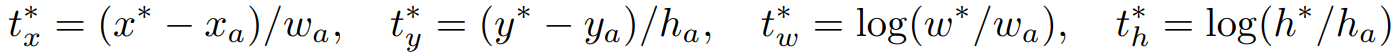
\includegraphics[width=400px]{rumus/regression_target.png}
   	\end{figure}
   
   	$x, y, w, h$ adalah koordinat (x, y) dari titik tengah kotak pembatas dan tinggi(h) dan lebar(w) kotak. $x^{*}, y^{*}, w^{*}, h^{*}$ adalah koordinat dan dimensi kotak-kotak groundtruth. Setiap "anchor" memiliki regresor yang berbeda, sehingga weight nya berbeda-beda. Ketika waktu pengujian, output regresi $t_{i}$ bisa diaplikasikan ke kotak "anchor", dan parameter $x, y, w, h$ untuk kotak pembatas prediksi bisa dihitung dari rumus :
   	
   	\begin{figure}[H]
   		\centering
   		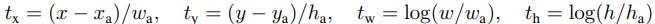
\includegraphics[width=400px]{rumus/regression_target_2.png}
   	\end{figure}
   	
   	\par Pada waktu pengujian, "anchors" dari setiap gambar melewati beberapa langkah post-processing untuk mengirimkan kotak-kotak pembatas objek.Koefisien regresi diaplikasikan ke "anchor" untuk lokalisasi yang tepat. Untuk kumpulan kotak-kota yang tumpang tindih, kotak yang memiliki IoU lebih dari 0.7 dengan kotak lain akan dibuang. Hanya proposal kotak pembatas sejumlah $n$ terbaik dari RPN akan dipilih.
   	
   	\begin{figure}[H]
   		\centering
   		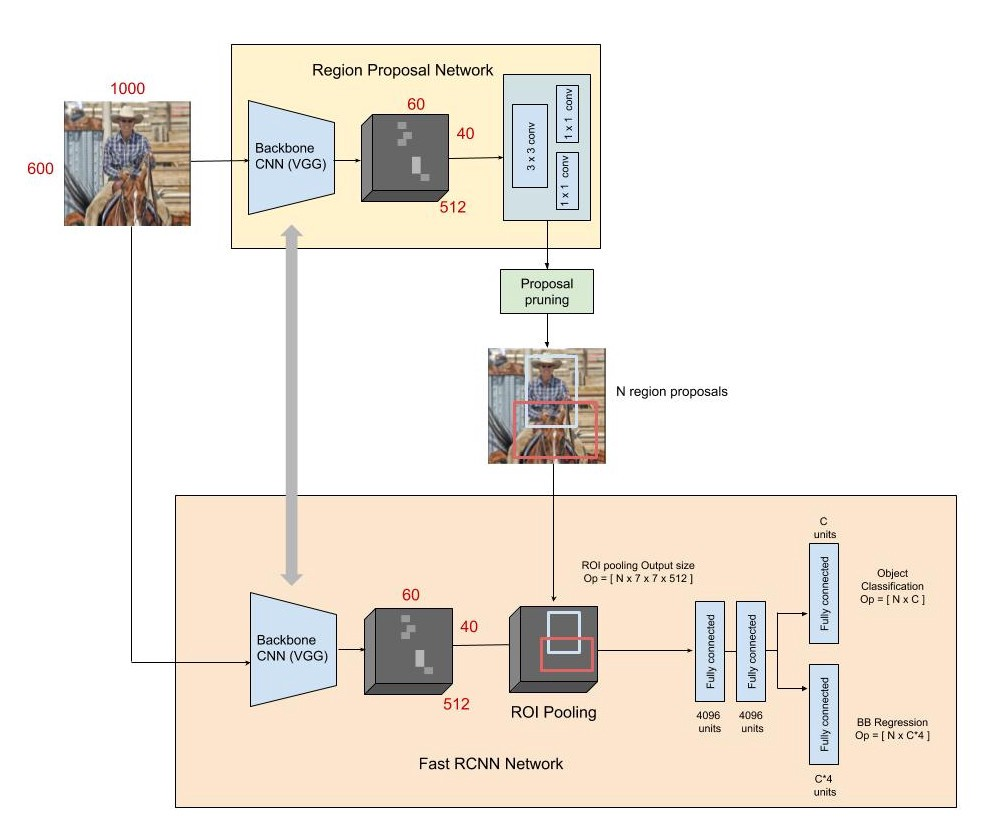
\includegraphics[width=400px]{arsitektur/full_architecture.jpeg}
   		\caption{Arsitektur Faster R-CNN Lengkap (RPN + Fast R-CNN)}
   	\end{figure}
   	
   	\par Arsitektur Faster R-CNN lengkap terdiri dari RPN sebagai algoritme proposal wilayah dan Fast R-CNN sebagai jaringan pendeteksi. Jaringan pendeteksi Fast R-CNN juga terdiri dari Backbone CNN, ROI pooling layer, dan fully-connected layer diikuti dengan dua cabang untuk klasifikasi dan regresi kotak pembatas. Gambar input dimasukkan ke Backbone CNN untuk mendapatkan feature map. Salah satu keuntungan menggunakan RPN sebagai penghasil proposal adalah pembagian weights antara backbone RPN dan backbone Fast R-CNN. Lalu, ROI pooling layer melakukan langkah-langkah di bawah :
   	\begin{enumerate}
   		\item Mengambil daerah proposal dari feature map backbone.
   		\item Membagi wilayah menjadi sub-wilayah dengan jumlah tertentu.
   		\item Melakukan max-pooling dari sub-wilayah untuk mendapatkan output dengan ukuran tertentu.
   	\end{enumerate}
   
   	\par Output ROI pooling layer dimasukkan ke dua fully-connected layer, lalu fitur-fitur dimasukkan ke cabang klasifikasi dan regresi. Cabang klasifikasi dan regresi berbeda dengan cabang klasifikasi dan regresi pada RPN. Disini classification layer memiliki $C$ unit untuk setiap kelas pada tugas deteksi. Fitur-fitur masuk melewati softmax layer untuk mendapatkan nilai klasifikasi, probabilitas proposal masuk ke dalam suatu kelas. Koefisien regresi digunakan untuk meningkatkan akurasi dari kotak pembatas. Setiap kelas memiliki regresor masing-masing dengan 4 parameter sesuai dengan $C$*4 unit output pada regression layer.
   	
   	\par Untuk memaksa jaringan untuk membagi weight Backbone CNN antara RPN dan Fast R-CNN, digunakan proses latihan 4 langkah :
   	\begin{enumerate}
   		\item RPN dilatih secara independen seperti penjelasan di atas.
   		\item Jaringan pendeteksi Fast R-CNN juga dilatih secara independen.
   		\item Weight RPN diinisialisasi dengan weight Faster R-CNN, lalu dilatih untuk tugas proposal wilayah. Weight pada lapisan-lapisan yang sama antara RPN dan Fast R-CNN tetap sama, hanya lapisan yang ada di RPN saja yang diubah.
   		\item Dengan menggunakan RPN baru, jaringan pendeteksi Fast R-CNN juga dilatih lagi. Hanya lapisan-lapisan yang ada di Fast R-CNN saja yang berubah weight nya. 
   	\end{enumerate}
   	
   	\begin{figure}[H]
   		\centering
   		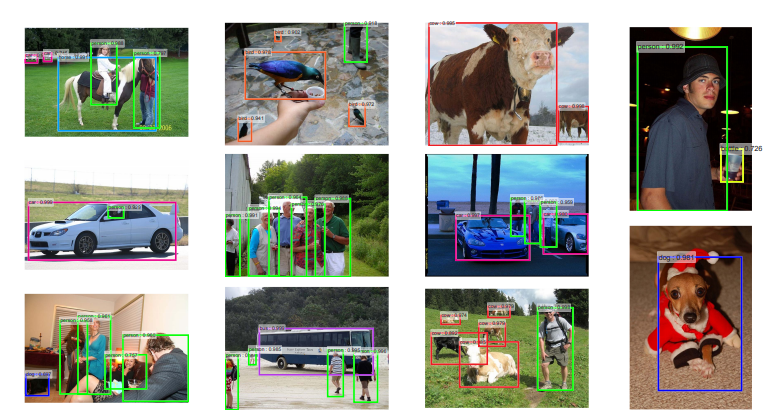
\includegraphics[width=400px]{arsitektur/contoh_hasil.png}
   		\caption{Hasil Faster R-CNN dengan Backbone VGG}
   	\end{figure}
   	
   	\newpage
  	\subsection{Implementasi Weight dari Faster R-CNN Model}
  	\subsubsection{Perangkat Uji Coba}
	\par Hasil output pembelajaran Faster R-CNN adalah \textit{weights} yang dapat digunakan secara langsung atau untuk memuat model dan memprediksi data baru dengan cepat. Untuk mengimplementasikan model secara langsung atau \textit{realtime} kami menggunakan perangkat keras : CPU Intel(R) i5-3470, GPU Nvidia GTX 960 2GB. Perangkat lunak dan \textit{libraries} : Python 3.7.7, mutils, OpenCV, pytorch, torchvision, numpy, pandas, dan ManyCam. 
	
	\par Dalam percobaan ini kami membuat 2 model program yang memiliki keunggulan masing-masing.
	\subsubsection{Program WebCam Pendeteksi Masker}
	\begin{figure}[H]
  		\centering
  		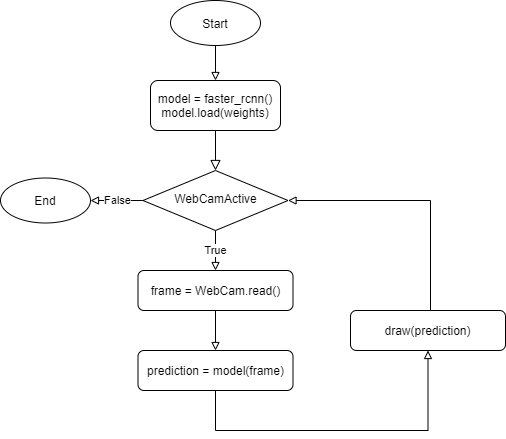
\includegraphics[width=200px]{arsitektur/Sequential Model.png}
  		\caption{Program WebCam Pendeteksi Masker Flowchart}
	\end{figure}
	Tugas dari program ini secara umum dapat dibagi menjadi 2 bagian : \\
	{\textbf{1. Proses Memuat \textit{Weights}}}
	\par Sebelum program dapat melakukan prediksi, model harus di inisialisasi atau dibuat terlebih dahulu dan selanjutnya model akan dimuat dengan \textit{Weights} yang ada dari hasil proses pembelajaran \textit{finetuning} Faster R-CNN.\\
	{\textbf{2. Looping ketika input WebCam Aktif}}
	\par Setelah model sudah siap untuk melakukan prediksi, akan dilakukan selama WebCam aktif maka program akan membaca input yang berasal dari WebCam tersebut dan menyampaikan input tersebut kepada model. Model akan melakukan \textit{Forward Pass} menghasilkan prediksi, informasi dari prediksi ini (labels, scores, boxes) akan digambarkan pada layar, setelah proses ini selesai maka program akan mengulang mengambil input baru sampai program di tutup oleh pengguna.\\
	\par Keuntungan dari program ini adalah kesederhanaannya, program ini mengandung seluruh elemen dasar yang dibutuhkan untuk membuat program deteksi \textit{realtime}.
	% \subsubsection{WebCam with Mutlithreaded Model}
  	% \begin{figure}[H]
  	% 	\centering
  	% 	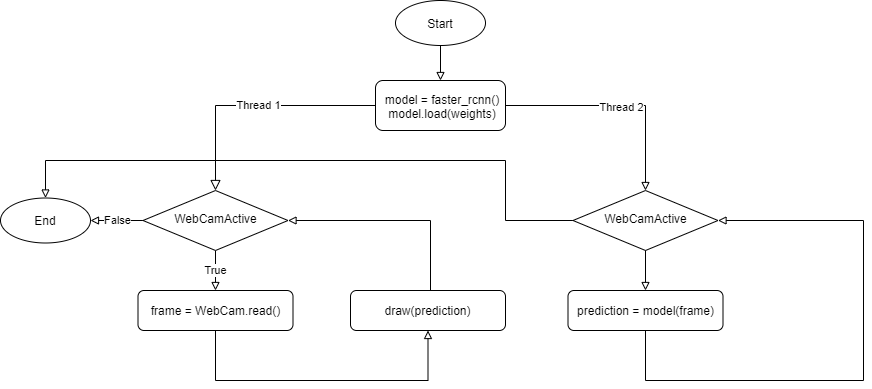
\includegraphics[width=400px]{arsitektur/Multithread Model.png}
  	% 	\caption{WebCam with Mutlithreaded Model Flowchart}
  	% \end{figure}
  	% Berdasarkan program dasar, program ini dapat dioptimalisasi performanya untuk terlihat lebih lancar dijalankan apabila update dari frame tidak bergantung atau terblokir menunggu hasil dari prediksi yang memakan cukup banyak waktu. Dengan menggunakan \textit{multithreading} prediksi dapat dilakukan secara asinkronus, membuat program terlihat lebih lancar. Dalam kasus ini kita dapat meminta \textit{thread 1} untuk melakukan input untuk prediksi dan langsung menggambarkan prediksi yang saat itu ada, sehingga \textit{thread 2} dapat di tugaskan untuk mengatur GPU membuat prediksi secepatnya. 
  	\subsubsection{Program WebCam Pendeteksi Masker dengan Post-processing}
  	\begin{figure}[H]
  		\centering
  		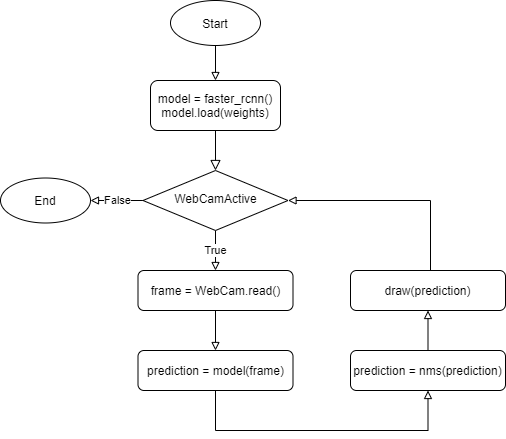
\includegraphics[width=200px]{arsitektur/Sequential with Postprocessing.png}
  		\caption{Program WebCam Pendeteksi Masker dengan Post-processing Flowchart}
	\end{figure}
	
	Kami mengusulkan program menggunakan post-processing \textit{non-maximum suppression} \cite{nms_pytorch} untuk memperjelas prediksi yang memiliki \textit{overlapping bounding box} dengan mengeliminasikan atau tidak memakai prediksi yang memiliki skor rendah dalam kotak yang sama. Hal ini terjadi karena perbedaan orang "memakai masker", "tidak memakai masker", dan "tidak memakai masker dengan baik" memiliki beberapa fitur yang sama seperti memiliki mata, bentuk wajah hal ini menyebabkan label terdeteksi tetapi memiliki skor yang rendah.\\

	\begin{figure}[H]
		\centering
		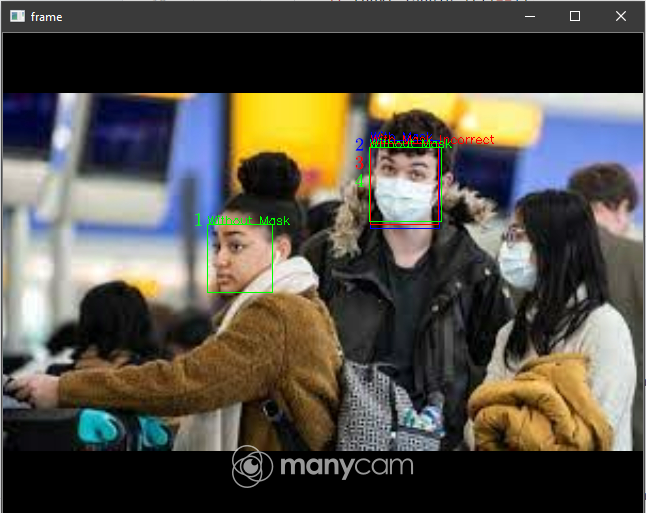
\includegraphics[width=250px]{../demo/Results/implementation/raw_prediction_nms0_labeled.png}
		\caption{Hasil prediksi program.}
	\end{figure}
	{\large{\textbf{Hasil Prediksi}}}
	\begin{table}[H]
		\centering
		\begin{tabular}{clc}
		\hline
		\textbf{i} & \textbf{Label}               & \textbf{Score}  \\ \hline
		1 & Without Mask        & \textbf{0.8836} \\
		2 & With Mask           & \textbf{0.8032} \\
		3 & With Mask Incorrect & 0.2569 \\
		4 & Without Mask        & 0.2145
		\end{tabular}
	\end{table}
	\newpage
	
	\begin{figure}[H]
		\centering
		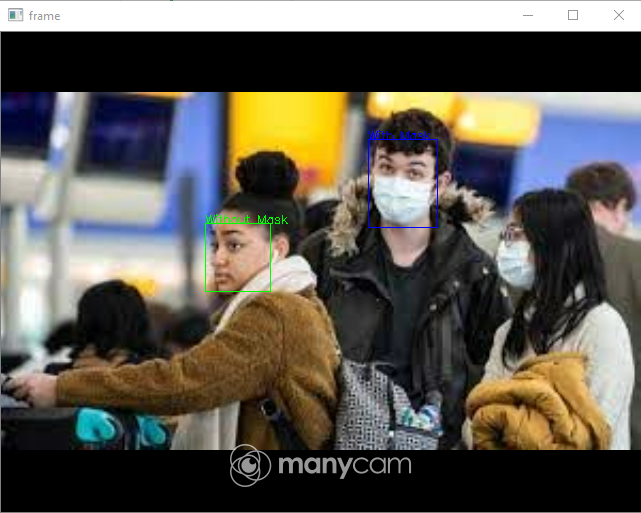
\includegraphics[width=250px]{../demo/Results/implementation/with_nms0.png}
		\caption{Hasil prediksi program dengan non-maximum suppression.}
  	\end{figure}
	{\large{\textbf{Hasil Prediksi Menggunakan Post-processing}}}
	\begin{table}[H]
		\centering
		\begin{tabular}{clc}
			\hline
			\textbf{i} & \textbf{Label}               & \textbf{Score}  \\ \hline
			1 & Without Mask        & \textbf{0.8836} \\
			2 & With Mask           & \textbf{0.8032} \\
		\end{tabular}
	\end{table}
  
  \section{Hasil}
  \section{Kesimpulan}
  	Ketika akan mengimplementasikan model ini maka infrastruktur atau alat yang dibutuhkan adalah sebuah cctv, (setidaknya) sebuah monitor, dan sebuah komputer. Pada hal ini komputer akan berguna sebagai alat untuk menghubungkan cctv dengan monitor dan menjadi tempat untuk model melakukan prediksi kepada gambar input. Kemudian cctv akan berguna menjadi alat untuk mendapatkan gambar input yang kemudian akan diprediksi oleh model. Cctv yang digunakan akan dihubungkan langsung dengan komputer dan gambar input dari cctv akan diproses frame by frame oleh model (Untuk sementara, tolong yg baca ingetin saya edit ini). Setelah itu monitor juga akan dihubungkan dengan komputer, monitor digunakan untuk menampilkan hasil dari input yang diambil dari cctv yang sudah didapatkan hasil prediksinya (ini juga). 
  	\begin{figure}[H]
  		\centering
  		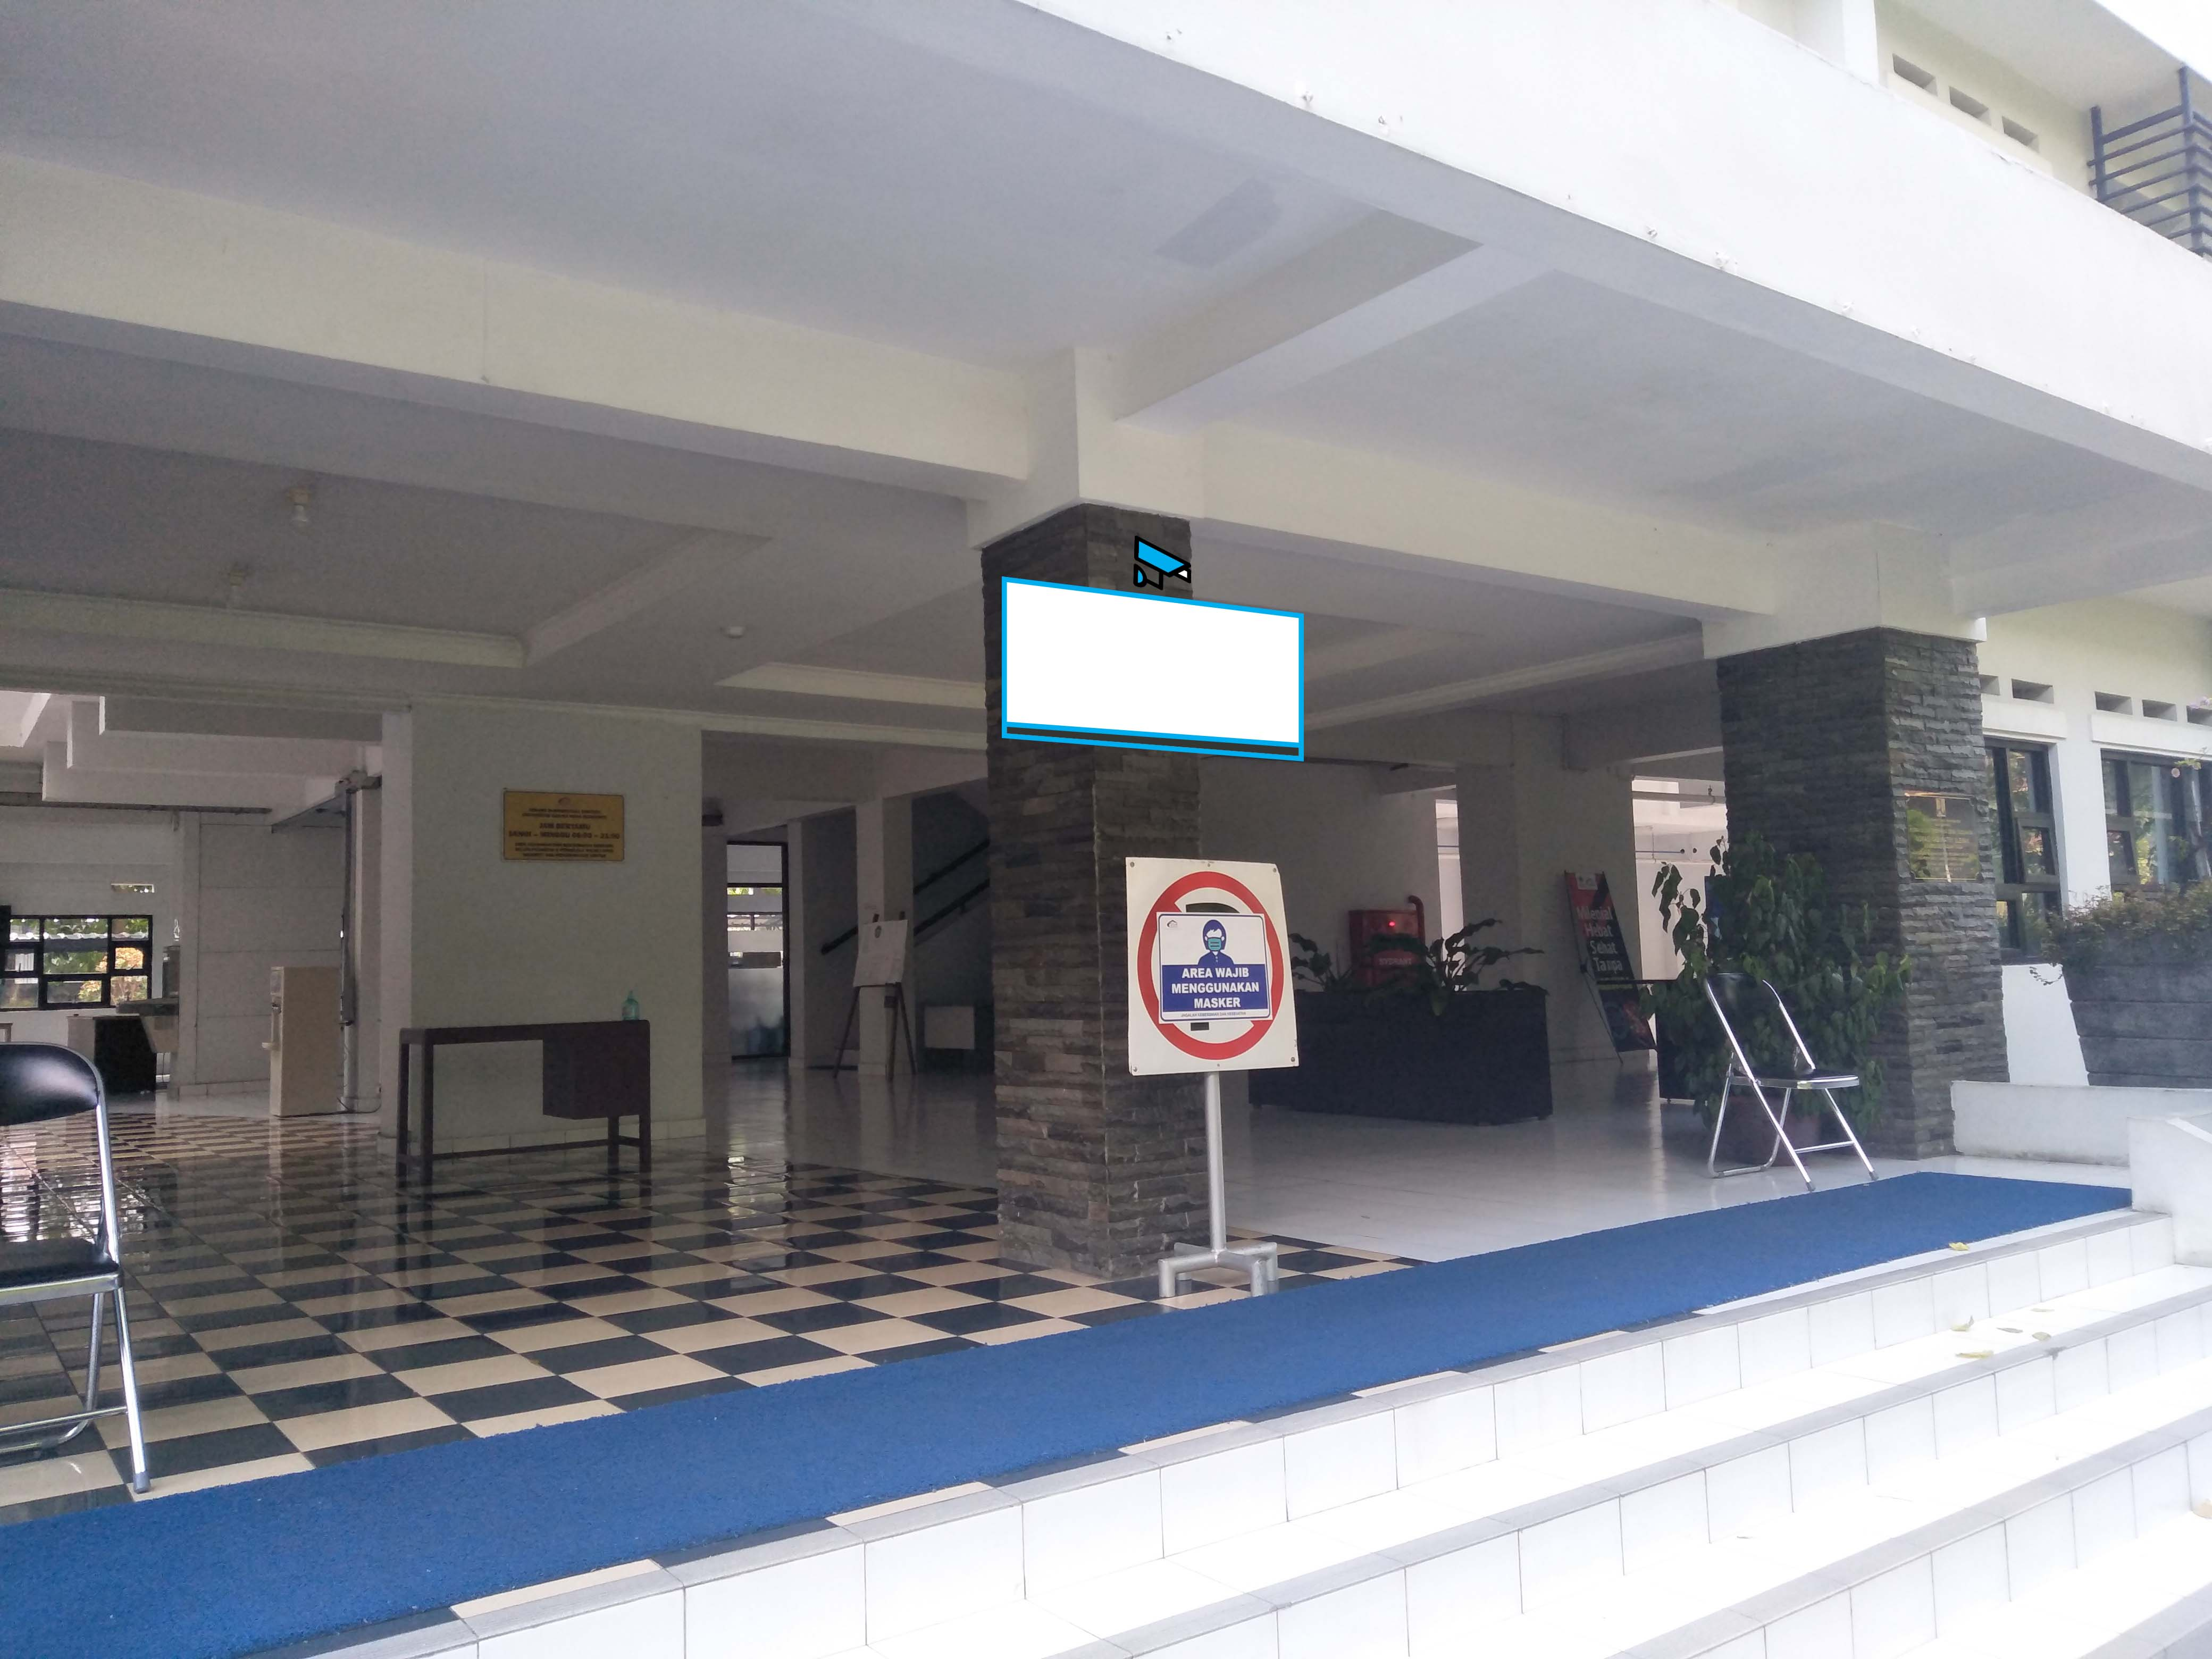
\includegraphics[width=400px]{implementasi/test.jpg}
  		\caption{Visualisasi Implementasi}
  	\end{figure}
	\par Untuk jumlah monitor sendiri tidak terbatas pada satu monitor saja, jumlah monitor dapat disesuaikan dan ditempatkan menyesuaikan dengan kebutuhan pada masing-masing tempat. Dalam monitor nanti gambar yang ditampilkan berdasarkan hasil prediksi setiap orang yang tertangkap dalam cctv akan diberikan bounding box sesuai dengan kategori yang cocok dengan mereka. (abis itu jelasin warna warna tiap kategori tp karena belom tau jadi ingetin nanti). Lalu jika dalam monitor terdapat orang-orang yang tidak menggunakan masker atau menggunakan masker dengan tidak benar maka pengawas/petugas yang berjaga disekitar dapat menegur orang-orang tersebut sesuai dengan kebijakan pada masing-masing tempat.
  \section{Lampiran}
  \newpage
  \printbibliography[title={Referensi}]
\end{document}